\documentclass[12pt]{article}

\usepackage[a4paper, left=1.2in, right=1.2in]{geometry}
\usepackage{setspace}
\usepackage[utf8]{inputenc}
\usepackage[italian]{babel}
\usepackage[OT1]{fontenc}
\usepackage{graphicx}
\usepackage{subcaption}
\usepackage{float}
\usepackage{fancyhdr}
\usepackage{xcolor}
\usepackage{mathtools}
\usepackage{amsmath}
\usepackage{amssymb}
\usepackage{tikz}
\usepackage{imakeidx}
\usepackage{textcomp}
\usepackage{pifont}
\usepackage{polynom}
\usepackage{algorithm}
\usepackage{algpseudocode}
\usepackage{mathtools}
\usepackage{cancel}
\usepackage{pgfplots}
\usepackage{caption}
\usepackage{tabularx}
\usepackage{comment}
\usepackage{float}
\usepackage{bm}
\usepackage{multirow}
\usepackage{listings}
\usepackage{longtable}
\usepackage[colorlinks=true,linkcolor=black,anchorcolor=black,citecolor=black,filecolor=black,menucolor=black,runcolor=black,urlcolor=black,backref=page]{hyperref}
\begin{document}


\lstset{ 
  language=Python,
  framesep=1pt,
  xleftmargin=0pt,
  framexleftmargin=0pt,
  frame=tb,
  framerule=1pt,
  breaklines=true,
  keywordstyle=\color{blue}\bfseries,
  showstringspaces=false
}

\lstset{ 
  language=SQL,
  morekeywords={AFTER, INSTEAD, OF, REFERENCING, FOR, EACH, ROW, DECLARE, IF, TYPE, NEW, RETURNS, SELF, BEGIN, END, CONSTRUCTOR, UNDER, CONSTRUCTOR, STATIC, INSTANCE, RETURN, OVERRIDING, FINAL, NOT, INSTANTIABLE, UNNEST, MULTISET, ARRAY, COLLECT, METHOD, REF, MEMBER, FUNCTION, PROCEDURE, PRAGMA, RESTRICT_REFERENCES, WNDS, RNDS, TABLE, WITH, ASSIGNMENT, OPTIONS, SCOPE, NESTED, STORE, DEREF, VARRAY, OBJECT, DBMS_OUTPUT, PUT_LINE, INSERTING, UPDATING, THEN, FOR, LOOP, EXTEND, REF, TRUNC, DBMS_RANDOM, TO_CHAR, TO_DATE, PROCEDURE, REPLACE, BEFORE, COMPOUND, OLD, RAISE_APPLICATION_ERROR, SYSDATE, STATEMENT, IS, ROUND, NVL, ELSIF, DUAL, RAWTOHEX, GUID, SYS},
  framesep=1pt,
  xleftmargin=0pt,
  framexleftmargin=0pt,
  frame=tb,
  framerule=1pt,
  breaklines=true,
  commentstyle=\color{deepgreen},
  keywordstyle=\color{deepblue},
  showstringspaces=false,
  mathescape
}
\renewcommand{\tablename}{Table}
\renewcommand{\figurename}{Figure}
\begin{titlepage}
    \begin{center}
        
\includegraphics[scale=0.5]{images/uniba-logo.png}\\
        \vspace{0.5cm}
        % Dipartimento
        {\large COMPUTER SCIENCE DEPARTMENT}\\
        \vspace{0.5cm}
        % Corso di laurea
        {\large Computer Science - Curriculum Artificial Intelligence}\\
        \hrulefill \\
        \vspace{0.5cm}
        {\large Project Assignment}\\
        \vspace{0.5cm}
        % Materia
        {\large Database Systems}\\
        \vspace{0.5cm}
        % Titolo
        {\LARGE \textbf{Database Design and Implementation}}\\
        %% \textbf{Titolo della Tesi} 
        \vspace{0.5cm}

        \vfill
        \centering
        \begin{tabularx}{\textwidth}{@{}Xr@{}}
          % Relatore
          {\large Student:} &
          {\large \textit{Fontana Emanuele}} \\ 
        \end{tabularx}
        \textcolor{white}{.} \\ 
        \vspace{0.5cm}
        \hrulefill \\
        % Anno accademico in cui si è iscritti
        {\large Academic Year 2024/2025}
    \end{center}
\end{titlepage}
\newpage
\tableofcontents
\newpage
\section{Conceptual Design}
\subsection{Requirements}
The requirements for the database are the following:
\begin{table}[H]
    \renewcommand{\arraystretch}{1.3} % Adjust row height
    \begin{tabularx}{\textwidth}{|X|}
    \hline
    \textbf{"GreenWorld Energy"} \\ \hline
    The company "GreenWorld Energy" operates decentralized renewable energy production facilities distributed 
across regions. Each facility is characterized by a name, location, type of energy produced (e.g., solar, wind, 
hydro), and maximum energy output capacity. The company also manages contracts with customers for energy 
supply, categorized as residential or commercial, and offers flexible pricing models based on consumption. 
Each customer has one or more accounts, each identified by a unique code. Every energy contract is linked to a 
single customer account and includes details such as start date, duration, energy plan, and cost. Facilities are 
overseen by management teams, each identified by a unique code, team name, and the number of projects managed. 
Teams are evaluated based on performance metrics such as energy efficiency, uptime, and customer satisfaction. 
Each team is represented by the main responsible employee and other employees identified by fiscal code, name, 
surname, date of birth and date of hiring. Additionally, the company supports a feedback system allowing 
customers to submit ratings and comments regarding service quality. Customers are classified into residential and 
commercial types, each identified by a unique alphanumeric code, with associated contact details and energy 
consumption history. \\ \hline
    \end{tabularx}
    \caption{Requirements}
    \end{table}


\subsection{Analysis}

\subsubsection{Glossary of Terms}
\begin{table}[H]
    \renewcommand{\arraystretch}{1.3} % Adjust row height
    \begin{tabularx}{\textwidth}{|X|X|X|X|}
    \hline
    \textbf{Term}& \textbf{Description}  & \textbf{Connections}    & \textbf{Synonyms}     \\ \hline
    Region      & Area where the facilities are located. & Facility     & Location \\ \hline
    Facility     & Energy production facility. It emits energy for customers      & Contract,Teams,Region         &\\ \hline
    Contract     & Energy supply contract. It describes the energy plan. It can be residential or commercial & Account, Facility     & Projects        \\ \hline
    Customer     & Customer of GreenWorld Energy. It can be residential or commercial       & Account    &        \\ \hline
    Account      & Customer account. It associated with only one account and one contract & Contract, Customer, Feedback     &        \\ \hline
    Feedback     & Customer feedback. Used to give a score to each team       & Account,Team     &         Ratings, customer satisfaction \\\hline
    Team        & Groups of employees that oversees a facility. Each team has a manager       & Facility, Employee, Feedback     &        \\ \hline
    Employee     & Employee of a GreenWorld Energy's team.      & Team     &        \\ \hline
    \end{tabularx}
    \caption{Glossary of Terms}
    \end{table}
\newpage
\subsubsection{Level of Abstraction}
By considering the synonyms of the terms, we can identify the level of abstraction of the terms. The terms can be classified as follows:
\begin{itemize}
    \item \textbf{Region} as Location
    \item \textbf{Facility} as Facility
    \item \textbf{Contract} as Contract
    \item \textbf{Customer} as Customer
    \item \textbf{Account} as Account
    \item \textbf{Feedback} as Feedback
    \item \textbf{Team} as Team
    \item \textbf{Employee} as Employee
\end{itemize}

\subsubsection{Reorganization of Concepts}
The concepts can be reorganized as follows:
\begin{table}[H]
    \renewcommand{\arraystretch}{1.3} % Adjust row height
    \begin{tabularx}{\textwidth}{|X|}
    \hline  \textbf{Facility}    \\ \hline
    Each facility is characterized by a name, location, type of energy produced (e.g., solar, wind, hydro), and maximum energy output capacity. The company also manages contracts with customers for energy supply, categorized as residential or commercial, and offers flexible pricing models based on consumption. Facilities are overseen by management teams \\ \hline
    \end{tabularx}
    \caption{Facility's Concepts}
    \end{table}

\begin{table}[H]
    \renewcommand{\arraystretch}{1.3} % Adjust row height
    \begin{tabularx}{\textwidth}{|X|}
    \hline  \textbf{Contract}    \\ \hline
    The company also manages contracts with customers for energy supply, categorized as residential or commercial, and offers flexible pricing models based on consumption.
    Every enegry contract is linked to a single customer account and includes details such as start date, duration, energy plan, and cost. \\ \hline
    \end{tabularx}
    \caption{Contract's Concepts}
    \end{table}

\begin{table}[H]
    \renewcommand{\arraystretch}{1.3} % Adjust row height
    \begin{tabularx}{\textwidth}{|X|}
    \hline  \textbf{Customer}    \\ \hline
    Each customer has one or more accounts, each identified by a unique code. Customers are classified into residential and commercial types, each identified by a unique alphanumeric code, with associated contact details and energy consumption history. Additionally, the company supports a feedback system allowing customers to submit ratings and comments regarding service quality. \\ \hline
    \end{tabularx}
    \caption{Customer's Concepts}
    \end{table}

\begin{table}[H]
    \renewcommand{\arraystretch}{1.3} % Adjust row height
    \begin{tabularx}{\textwidth}{|X|}
    \hline   \textbf{Account}    \\ \hline
    Each customer has one or more accounts, each identified by a unique code. Every energy contract is linked to a single customer account and includes details such as start date, duration, energy plan, and cost. \\ \hline
    \end{tabularx}
    \caption{Account's Concepts}
    \end{table}

\begin{table}[H]
    \renewcommand{\arraystretch}{1.3} % Adjust row height
    \begin{tabularx}{\textwidth}{|X|}
    \hline  \textbf{Feedback}    \\ \hline
    The company supports a feedback system allowing customers to submit ratings and comments regarding service quality. \\ \hline
    \end{tabularx}
    \caption{Feedback's Concepts}
    \end{table}

\begin{table}[H]
    \renewcommand{\arraystretch}{1.3} % Adjust row height
    \begin{tabularx}{\textwidth}{|X|}
    \hline  \textbf{Team}    \\ \hline
    Facilities are overseen by management teams, each identified by a unique code, team name, and the number of projects managed. Teams are evaluated based on performance metrics such as energy efficiency, uptime, and customer satisfaction. Each team is represented by the main responsible employee \\ \hline
    \end{tabularx}
    \caption{Team's Concepts}
    \end{table}

\begin{table}[H]
    \renewcommand{\arraystretch}{1.3} % Adjust row height
    \begin{tabularx}{\textwidth}{|X|}
    \hline  \textbf{Employee}    \\ \hline
    Each team is represented by the main responsible employee and other employees identified by fiscal code, name, surname, date of birth and date of hiring. \\ \hline
    \end{tabularx}
    \caption{Employee's Concepts}
    \end{table}

\subsubsection{Entity-Relationship Diagram}

\paragraph{SKELETON SCHEMA} \leavevmode \newline
\begin{figure}[H]
    \centering
    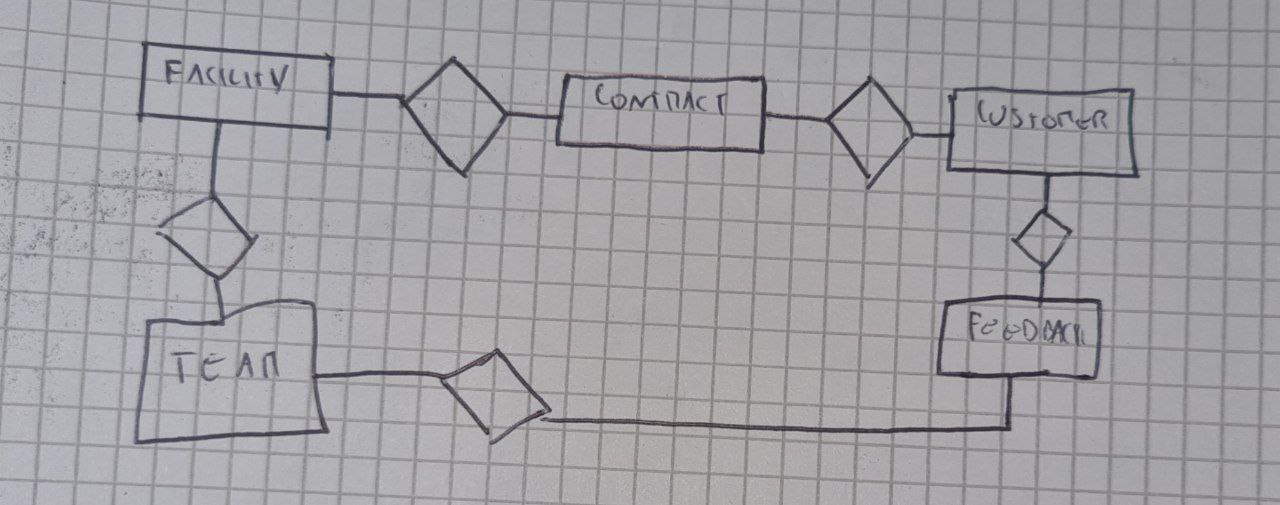
\includegraphics[width=\textwidth]{images/SkeletonSchema.png}
    \caption{Skeleton Schema}
\end{figure}

\noindent This schema represents the main entities and their relationships. The entities are the following:
\begin{itemize}
    \item \textbf{Facility}
    \item \textbf{Contract}
    \item \textbf{Customer}
    \item \textbf{Feedback}
    \item \textbf{Team}
\end{itemize}
The purpose of this schema is to have a general idea of the entities and their relationships. The attributes of the entities and the cardinality of the relationships are not included in this schema. Also, some entities are not included in this schema, such as Account and Employee. These entities will be included in the final schema with all the other details.

\paragraph{FINAL SCHEMA} \leavevmode \newline

\begin{figure}[H]
    \centering
    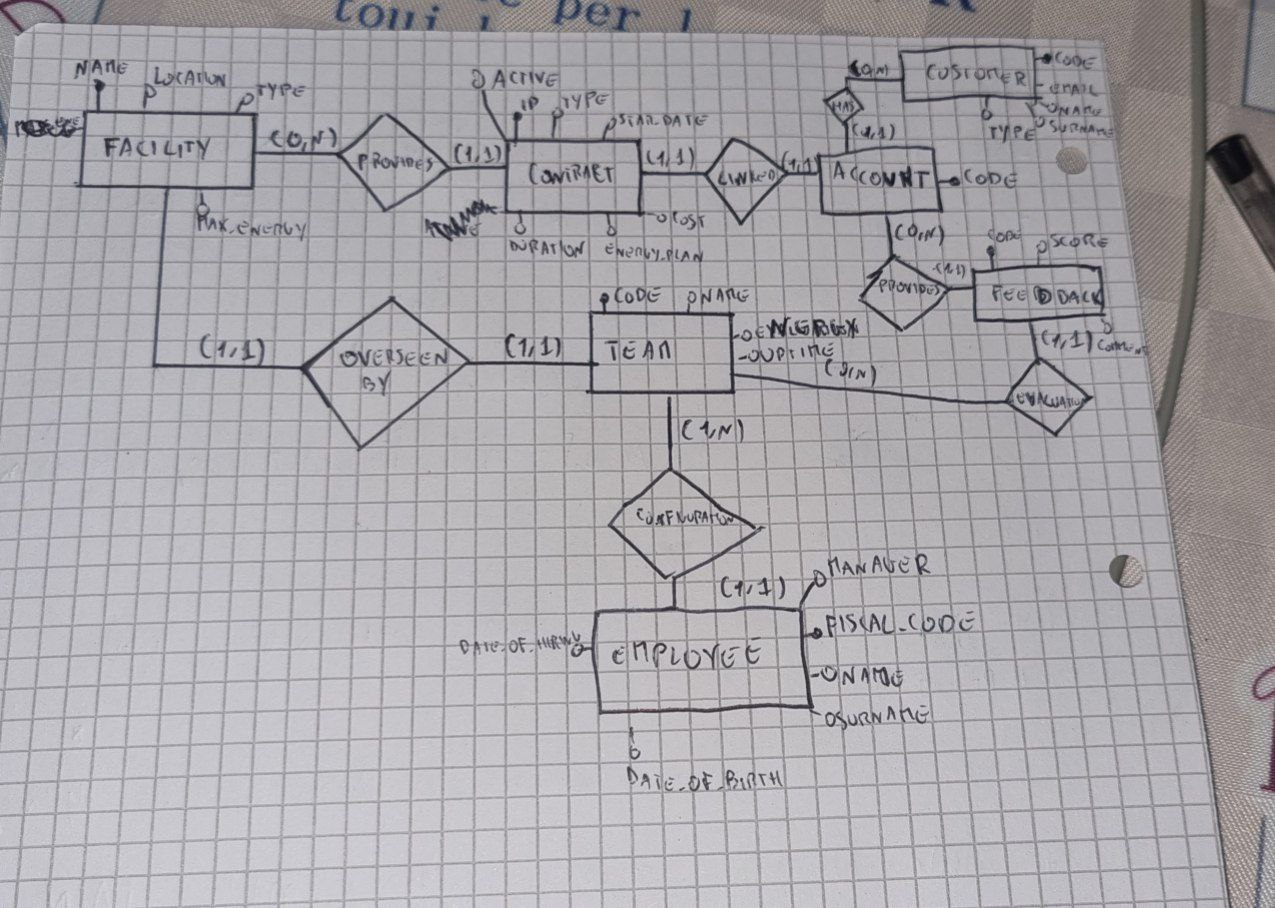
\includegraphics[width=\textwidth]{images/ER.png}
    \caption{Final Schema}
\end{figure}


\subsubsection{Business Rules}
The business rules are the following:
\begin{itemize}
    \item A customer can't be a minor
    \item An employee can't be a minor
    \item Each team has got only one main responsible employee
    \item The sum of energy plan of all contracts related to a facility can't exceed the maximum energy output capacity of the facility
    \item If an account needs to activate a new contract with the same facility, the old contract must deactivated before the new one is activated
    \item A customer of a specific type can't have a contract of the other type
    \item The score of a feedback can be between 0 and 5
    \item Uptime is the number of hours the facility is active in a day. Between 6 and 8
    \item Energy efficiency is the percentage of energy produced compared to the maximum energy output capacity of the facility. Between 0 and 100
\end{itemize}




\newpage
\section{Logical Design}

\subsection{Volume Table}
Lets consider the volumes for a year

\begin{table}[H]
    \scriptsize
    \renewcommand{\arraystretch}{1.3} % Adjust row height
    \begin{tabularx}{\textwidth}{|X|X|X|X|}
    \hline
    \textbf{Concept}& \textbf{Type}  & \textbf{Volume}    & \textbf{Description}     \\ \hline
    Facility & E & 100 & Number of facilities (Given) \\ \hline
    Contract & E & 900.000 & Number of contracts. 100 facilities * 500 contracts per facility * 12 months * 1.5 contracts per account \\ \hline
    Customer & E & 300.000 & Number of customers.(ASSUMPTION) \\ \hline
    Account & E & 600.000 & Number of accounts. 300.000 customers * 2 accounts per customer on average\\ \hline
    Team & E & 50 & Number of teams. (ASSUMPTION) \\ \hline
    Employee & E & 250 & Number of employees. 5 employees per team * 50 teams (ASSUMPTION) \\ \hline
    Feedback & E & 600.000 & Number of feedbacks.\\ \hline
    Provides & R & 900.000 & Each contract is provided by a single facility \\ \hline
    Linked & R & 900.000 & On average each account has 1.5 contracts \\ \hline
    Has & R & 600.000 & Each customer 2 accounts on average \\ \hline
    OverseenBy & R & 100 & Each facility is overseen by a single team. Each team oversees 2 facilities, on average \\ \hline
    Configuration & R & 500 & Each team constists of 5 employees on average \\ \hline
    Gives & R & 500.000 & Each feedback is given by a single account.Not all accounts give feedback  \\ \hline
    Evaluation & R & 500.000 & Each feedback is linked to a single team\\ \hline
    \end{tabularx}
    \caption{Volume Table}
\end{table}

\subsection{Access Table}

\textbf{Operation1:} Register a new customer (50 times per day)\\
\begin{table}[H]
    \renewcommand{\arraystretch}{1.3} % Adjust row height
    \begin{tabularx}{\textwidth}{|X|X|X|X|}
    \hline
    \textbf{Concept}& \textbf{Type}  & \textbf{Access}    & \textbf{Type}     \\ \hline
    Customer & E & 1 & W \\ \hline
    \end{tabularx}
    \caption{Access Table for Operation1}
\end{table}
\noindent Total Cost: 2 * 50 = 100 per day
\newline
\textbf{Operation2:} Register a new energy contract (50 times per day)\\
\begin{table}[H]
    \renewcommand{\arraystretch}{1.3} % Adjust row height
    \begin{tabularx}{\textwidth}{|X|X|X|X|}
    \hline
    \textbf{Concept}& \textbf{Type}  & \textbf{Access}    & \textbf{Type}     \\ \hline
    Contract & E & 1 & W \\ \hline
    Provides & R & 1 & W \\ \hline
    Facility & E & 1 & R \\ \hline
    Linked & R & 1 & W \\ \hline
    Account & E & 1 & R \\ \hline
    Facility & E & 1 & W \\ \hline
    Provides & R & 9000 & R \\ \hline
    Contract & E & 9000 & R \\ \hline
    \end{tabularx}
    \caption{Access Table for Operation2}
\end{table}
\noindent Total Cost: (2+2+1+2+1+2+9000+9000)*200=3.602.000 per day

\noindent Every time we need to update the efficiency score of the facility related to the contracts.
\newline
\noindent \textbf{Operation3:} Assign a facility to a management team (50 times per day)\\
\begin{table}[H]
    \renewcommand{\arraystretch}{1.3} % Adjust row height
    \begin{tabularx}{\textwidth}{|X|X|X|X|}
    \hline
    \textbf{Concept}& \textbf{Type}  & \textbf{Access}    & \textbf{Type}     \\ \hline
    Team & E & 1 & R \\ \hline
    OverseenBy & R & 1 & W \\ \hline
    Facility & E & 1 & R \\ \hline
    \end{tabularx}
    \caption{Access Table for Operation3}
\end{table}
\noindent Total Cost: (1+2+1)*50=200 per day
\newline
\noindent \textbf{Operation4:} View the total energy output of a specific facility managed by the eldest employee (1 per month = 0.03 per day)\\
\begin{table}[H]
    \renewcommand{\arraystretch}{1.3} % Adjust row height
    \begin{tabularx}{\textwidth}{|X|X|X|X|}
    \hline
    \textbf{Concept}& \textbf{Type}  & \textbf{Access}    & \textbf{Type}     \\ \hline
    Employee & E & 250 & R \\ \hline
    Configuration & R & 1 & R \\ \hline
    Team & E & 1 & R \\ \hline
    OverseenBy & R & 2 & R \\ \hline
    Facility & E & 2 & R \\ \hline
    Provides & R & 9000 & R \\ \hline
    Contract & E & 9000 & R \\ \hline
    \end{tabularx}
    \caption{Access Table for Operation4}
\end{table}
\noindent Total Cost: (250+1+1+1+2+9000+9000)*0.03=547.65 per day
\newline
\noindent Each team oversees, on average, twow facilities. We need to choose only one of them, which provides on average 9000 contracts.
In this case we don't have sumEnergyOutput in the schema as attribute of the facility, so we need to compute it every time. If we introduce it, the cost will be
\begin{table}[H]
    \renewcommand{\arraystretch}{1.3} % Adjust row height
    \begin{tabularx}{\textwidth}{|X|X|X|X|}
    \hline
    \textbf{Concept}& \textbf{Type}  & \textbf{Access}    & \textbf{Type}     \\ \hline
    Employee & E & 250 & R \\ \hline
    Configuration & R & 1 & R \\ \hline
    Team & E & 1 & R \\ \hline
    OverseenBy & R & 2 & R \\ \hline
    Facility & E & 2 & R \\ \hline
    \end{tabularx}
    \caption{Access Table for Operation4 with redundancy}
\end{table}
\noindent Total Cost: (250+1+1+2+2)*0.03=7.68 per day
\newline
\noindent But in this case we need to update it every time we add a new contract, so the total cost of \textbf{Operation2} will be:

\begin{table}[H]
    \renewcommand{\arraystretch}{1.3} % Adjust row height
    \begin{tabularx}{\textwidth}{|X|X|X|X|}
    \hline
    \textbf{Concept}& \textbf{Type}  & \textbf{Access}    & \textbf{Type}     \\ \hline
    Contract & E & 1 & W \\ \hline
    Provides & R & 1 & W \\ \hline
    Facility & E & 1 & R \\ \hline
    Facility & E & 1 & W \\ \hline
    Linked & R & 1 & W \\ \hline
    Account & E & 1 & R \\ \hline
    Facility & E & 1 & W \\ \hline
    Provides & R & 9000 & R \\ \hline
    Contract & E & 9000 & R \\ \hline
    \end{tabularx}
    \caption{Access Table for Operation2 with redundancy}
\end{table}
\noindent Total Cost: (2+2+1+2+2+1+2+9000+9000)*200=3.602.400 per day
\newline
\noindent So the total cost without redundancy is 3.602.000 +547.65 = 3.602.547.65, while the total cost with redundancy is 3.602.400 + 7.68 = 3.602.407.68 per day. So we should keep the redundancy in this case. 
\newline
\noindent \textbf{Operation5:} Print a ranked list of facilities based on their efficiency scores (10 per day)
\begin{table}[H]
    \renewcommand{\arraystretch}{1.3} % Adjust row height
    \begin{tabularx}{\textwidth}{|X|X|X|X|}
    \hline
    \textbf{Concept}& \textbf{Type}  & \textbf{Access}    & \textbf{Type}     \\ \hline
    Facility & E & 100 & R \\ \hline
    \end{tabularx}
    \caption{Access Table for Operation5}
\end{table}
\noindent Total Cost: 100*10 = 1000 per day

\noindent We can try to remove the redundancy of the efficiencyScore in facilities
\begin{table}[H]
\renewcommand{\arraystretch}{1.3} % Adjust row height
\begin{tabularx}{\textwidth}{|X|X|X|X|}
\hline
\textbf{Concept}& \textbf{Type}  & \textbf{Access}    & \textbf{Type}     \\ \hline
Facility & E & 100 & R \\ \hline
Provides & R & 900.000 & R \\ \hline
Contract & E & 900.000 & R \\ \hline
\end{tabularx}
\caption{Access Table for Operation5 without redundancy}
\end{table}
\noindent Total Cost: (100+900.000+900.000)*10 = 18.001.000 per day 
\begin{table}[H]
    \renewcommand{\arraystretch}{1.3} % Adjust row height
    \begin{tabularx}{\textwidth}{|X|X|X|X|}
    \hline
    \textbf{Concept}& \textbf{Type}  & \textbf{Access}    & \textbf{Type}     \\ \hline
    Contract & E & 1 & W \\ \hline
    Provides & R & 1 & W \\ \hline
    Facility & E & 1 & R \\ \hline
    Linked & R & 1 & W \\ \hline
    Account & E & 1 & R \\ \hline
    \end{tabularx}
    \caption{Access Table for Operation2 without redundancy}
\end{table}
\noindent Total Cost: (2+2+1+2+1)*200=1.600 per day
\newline
\noindent Now we don't need to update the the efficiency score everytime we register a new contract.

\noindent So the total cost without redundancy is 18.002.600, while the total cost with redundancy is 2.402.000 + 1000 = 2.403.000 per day.

\noindent We shouuld keep the redundancy in this case.

\subsubsection{Redundancies and Generalization}
\begin{itemize}
    \item \textbf{Redundancies:} The number of facilities managed by a team is not stored in the schema, as it can be calculated by counting the number of facilities managed by the team. The score of the team can be derived by the following formula: $score = \frac{energy\_efficiency + uptime + AVG(customer\_score)}{3}$ and is not stored in the schema to avoid redundancy. Due to the previous analysis, the redundancy of the efficiency score and sumEngergyOutput in the facility are kept in the schema
    \item \textbf{Generalization:} The schema doesn't contain any generalization since there aren't different operations for them. There is a \textbf{type} attribute in the \textbf{Customer} and \textbf{Contract} entities so that the business rule related to the type of contract can be enforced.
\end{itemize}


\subsection{UML Schema}

\begin{figure}[H]
    \centering
    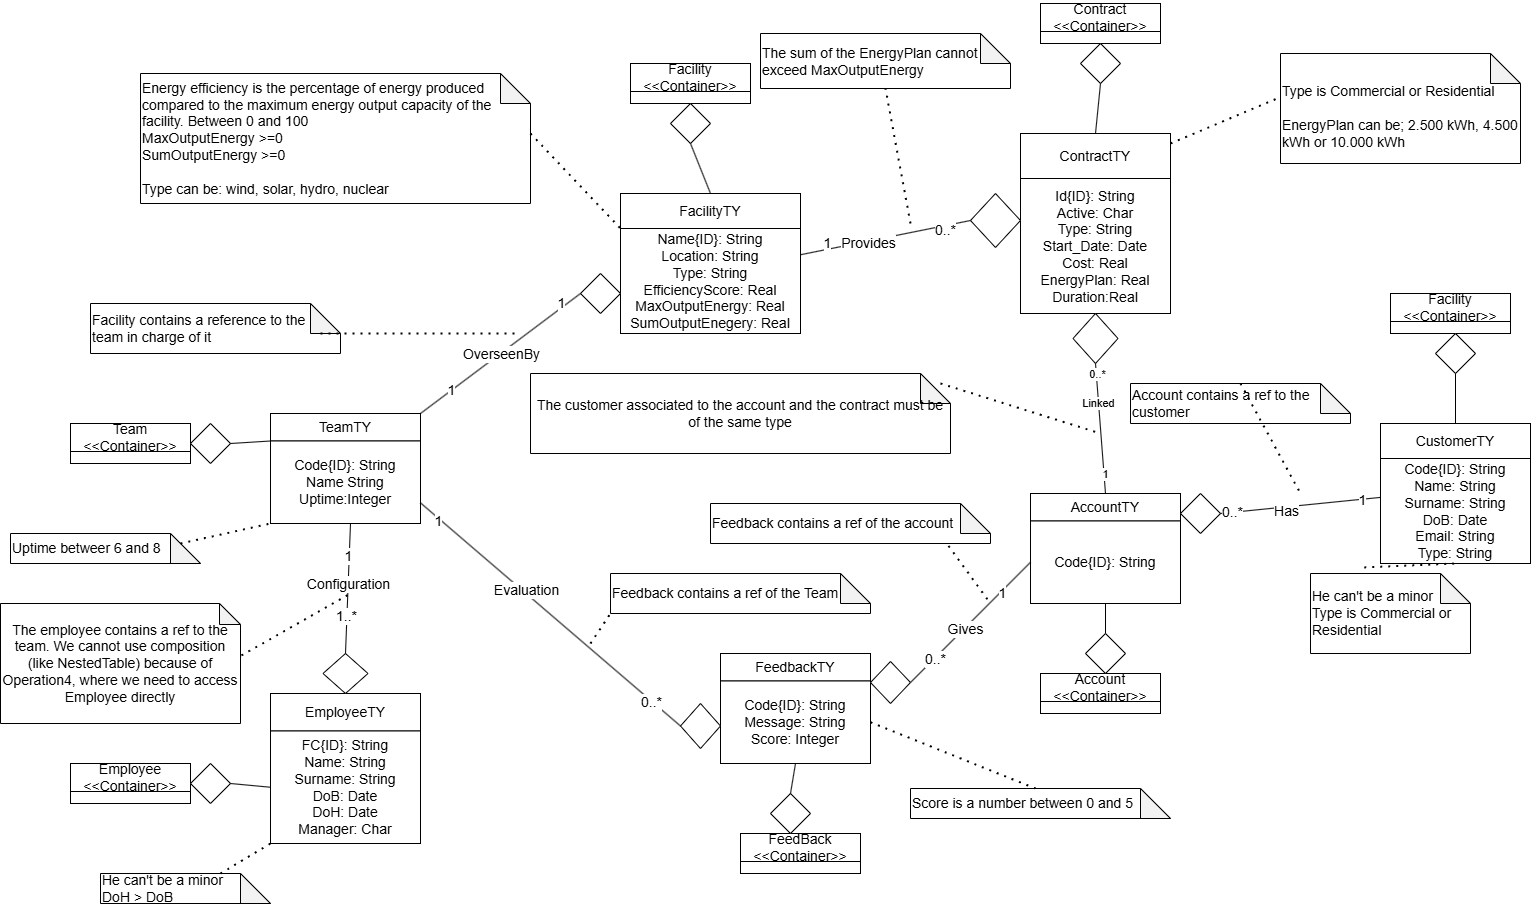
\includegraphics[width=\textwidth]{images/UML.png}
    \caption{UML Schema}
\end{figure}

\newpage
\section{Datawarehouse}

Here's a possible star-schema for the data warehouse:


\begin{figure}[H]
    \centering
    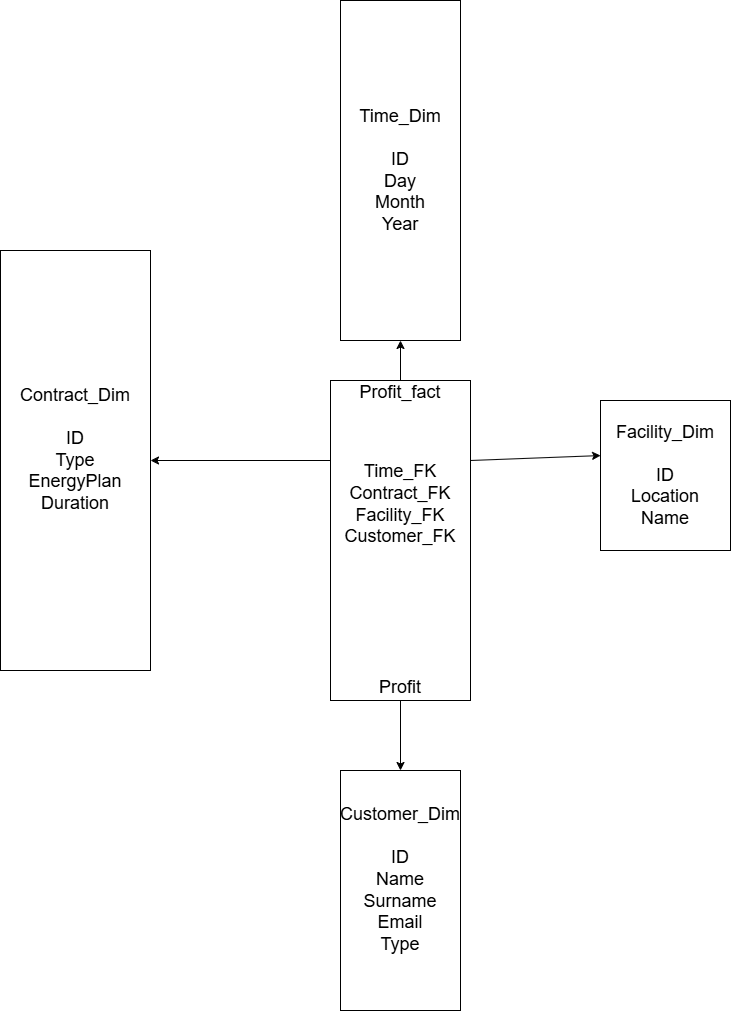
\includegraphics[width=\textwidth,height=0.7\textheight]{images/Fact1.png}
    \caption{Fact: Profit}
\end{figure}

\noindent In this example the main fact is the profit. We can analize it in different ways. Examples:
\begin{itemize}
    \item Profit by type of contract: what type of contract is more profitable?
    \item Profit by customer: who are the most profitable customers?
    \item Profit by Facility: which facilities are more profitable?
    \item Combined analysis: what type of contract is more profitable for a specific facility?
\end{itemize}

\begin{figure}[H]
    \centering
    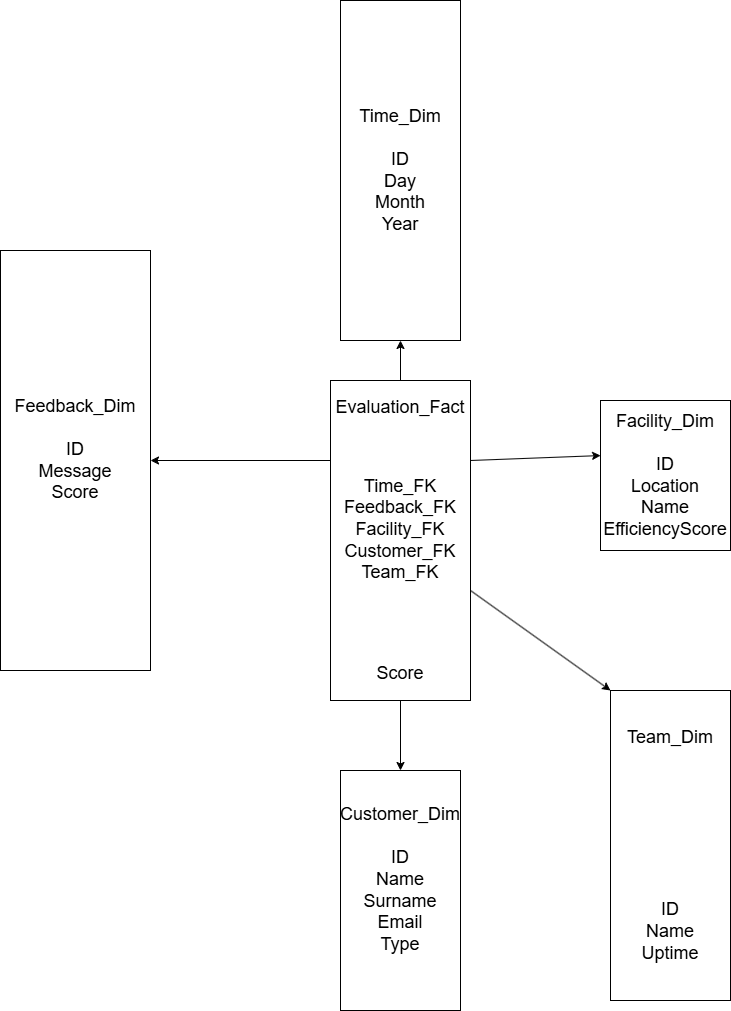
\includegraphics[width=\textwidth,height=0.7\textheight]{images/Fact2.png}
    \caption{Fact: Evalutation}
\end{figure}

\noindent In this example the main fact is the evaluation. We can analize it in different ways. Examples:
\begin{itemize}
    \item Which team has the best score? And the worst?
    \item On average, which component has the higher weight in the evaluation: energy efficiency, uptime, customer satisfaction?
    \item Combined analysis: what is the average evaluation of a customer?
    \item Combined analysis: has a customer have a bias in the evaluation of a specific team?
\end{itemize}

\end{document}